\documentclass[a4paper,12pt]{article}

\usepackage{comment}
\usepackage{supertabular}
\usepackage{graphics}
\usepackage{color,soul}
\usepackage{booktabs}
\usepackage{paralist}
\usepackage{algorithmicx}
\usepackage{algorithm}
\usepackage[noend]{algpseudocode}
\usepackage{booktabs}
\usepackage{hvfloat}
\usepackage{comment}
\usepackage{chngpage}
\usepackage{url}
\usepackage[utf8]{inputenc}
\usepackage[table,dvipsnames]{xcolor}
\usepackage[a4paper,pdftex,hmargin=0.75in,vmargin={1.1in,0.6in},head=75pt,foot=45pt, left=2.5cm, right=2.5cm, includefoot, footskip=60pt]{geometry}
\usepackage{lipsum}
\usepackage{afterpage}
\usepackage{xcolor}
\usepackage{tabularx}
\usepackage{wallpaper}
\usepackage{adjustbox}
\usepackage[normalem]{ulem}
\useunder{\uline}{\ul}{}
\usepackage{rotating}
\usepackage{parskip}
\usepackage{listings}
\lstset{language=C,breaklines=true}
\usepackage[english]{babel}
\usepackage{amsmath}
\usepackage{amsfonts}
\usepackage{amssymb}
\usepackage{amsthm}
\usepackage[justification=justified]{caption}
\usepackage{fontenc}
\usepackage[colorlinks=true]{hyperref}
\usepackage{multicol}
\usepackage{multirow}
\usepackage{array}
\usepackage{relsize}
\usepackage{subcaption}
\usepackage{caption}
\usepackage{tcolorbox}
\usepackage{lscape}
\usepackage{lastpage}
\usepackage{acro}
\setlength{\headsep}{1.5cm}
\usepackage[toc,page]{appendix}
\usepackage[nottoc]{tocbibind} % for show references in toc
\usepackage{pgfgantt}
\usepackage{tcolorbox}
\usepackage{thmtools}
\usepackage{physics}
\usepackage{cleveref}
\usepackage{calc}
\usepackage{cancel}
\frenchspacing
%\usepackage{svg}
%\usepackage{showframe}% for show page layout


\colorlet{LightGray}{White!90!Periwinkle}
\colorlet{LightOrange}{Orange!15}
\colorlet{LightGreen}{Green!15}

\newcommand{\HRule}[1]{\rule{\linewidth}{#1}}

\newtheorem{theorem}{Theorem}[section]

% \declaretheoremstyle[name=Theorem,]{thmsty}
% \declaretheorem[style=thmsty,numberwithin=section]{theorem}
% \tcolorboxenvironment{theorem}{colback=LightGray}

\declaretheoremstyle[name=Proposition,]{prosty}
\declaretheorem[style=prosty,numberlike=theorem]{proposition}
% \tcolorboxenvironment{proposition}{colback=LightOrange}

% \declaretheoremstyle[name=Principio,]{prcpsty}
% \declaretheorem[style=prcpsty,numberlike=theorem]{principle}
% \tcolorboxenvironment{principle}{colback=LightGreen}

% \newtheorem{corollary}{Corolario}[theorem]
% \newtheorem{lemma}[theorem]{Lema}
% \newtheorem{definition}{Definición}

% \tcolorboxenvironment{definition}{colback=LightGray}
%
\colorlet{punct}{red!60!black}
\definecolor{background}{HTML}{EEEEEE}
\definecolor{delim}{RGB}{20,105,176}
\colorlet{numb}{magenta!60!black}
\lstdefinelanguage{json}{
    basicstyle=\normalfont\ttfamily,
    numbers=left,
    numberstyle=\scriptsize,
    stepnumber=1,
    numbersep=8pt,
    showstringspaces=false,
    breaklines=true,
    frame=lines,
    backgroundcolor=\color{background},
    literate=
     *{0}{{{\color{numb}0}}}{1}
      {1}{{{\color{numb}1}}}{1}
      {2}{{{\color{numb}2}}}{1}
      {3}{{{\color{numb}3}}}{1}
      {4}{{{\color{numb}4}}}{1}
      {5}{{{\color{numb}5}}}{1}
      {6}{{{\color{numb}6}}}{1}
      {7}{{{\color{numb}7}}}{1}
      {8}{{{\color{numb}8}}}{1}
      {9}{{{\color{numb}9}}}{1}
      {:}{{{\color{punct}{:}}}}{1}
      {,}{{{\color{punct}{,}}}}{1}
      {\{}{{{\color{delim}{\{}}}}{1}
      {\}}{{{\color{delim}{\}}}}}{1}
      {[}{{{\color{delim}{[}}}}{1}
      {]}{{{\color{delim}{]}}}}{1},
}

%RBG FFD33E / C95D40
\definecolor{upcorange}{HTML}{FFD33E}
\hypersetup{allcolors=black}

% probably a good idea for the nomenclature entries:
\acsetup{first-style=short}

%%%% PAGE STYLE %%%%%
\usepackage{fancyhdr}
\pagestyle{fancy}
\fancyhf{}
\lhead{
\includegraphics[height=1.2cm]{img/logos/upclogo.png}}
\rhead{
\includegraphics[height=1.2cm]{img/logos/logo_telecos.png}}
\rfoot{\thepage{}}

\renewcommand{\footrulewidth}{0.4pt}
%\futurelet\TMPfootrule\def\footrule{{\color{upcorange}\TMPfootrule}}
\futurelet\TMPfootrule\def\footrule{{\color{gray!80}\TMPfootrule}}
\renewcommand{\headrulewidth}{0.4pt}
\renewcommand{\headrule}{\hbox to\headwidth{%
% \color{upcorange}\leaders\hrule height \headrulewidth\hfill}} % change color of top line
\color{gray!80}\leaders\hrule height \headrulewidth\hfill}}
%\renewcommand*\ShowFrameColor{\color{red}}

\renewcommand\theequation{\thesubsection.\arabic{equation}}

% class `abbrev': abbreviations:
\DeclareAcronym{EU}{
  short = EU ,
  long  = European Union ,
  tag = abbrev % class
}

\DeclareAcronym{ETSETB}{
  short = ETSETB ,
  long  = Escola Tècnica Superior d'Enginyeria de Telecomunicació de Barcelona ,
  % long = Barcelona School of Telecommunications Engeneering ,
  tag = abbrev % class
}



\begin{document}

%%% COVER %%%
\fancypagestyle{alim}{\fancyhf{}\renewcommand{\headrulewidth}{0pt}
\cfoot{
\includegraphics[height=2.2cm]{img/logos/logo_telecos.png}}
}
\thispagestyle{empty}
\begin{center}
{\sffamily 
\resizebox{0.8\textwidth}{!}{
\includegraphics{img/logos/upc_completo+telecos.png}}\\
\vspace{1cm}
{\Huge Disordered quantum gases}\\
\vspace{0.5cm}
{\color{black}\hrule height 1pt}
\vspace{1cm}
{\large{Master Thesis\\
submitted to the Faculty of the \\
Escola T\`ecnica d'Enginyeria de Telecomunicaci\'o de Barcelona \\
Universitat Polit\`ecnica de Catalunya \\
by\\
\vspace{0.4cm}
Pau Fargas Reixats}}

\nocite{*} % only if you no use \cite{}

\vspace{1.5cm}

{In partial fulfillment\\
of the requirements for the master in\\
\textit{Physics} \textbf{ENGINEERING}}

\vspace{2cm}

{{Advisor: Dr. Pietro Massignan}} \\
{{Barcelona, Date XXXXX}}
\thispagestyle{alim}
}

%%% INDEX %%%
\end{center}
\newpage
\tableofcontents

%%% LISTS %%%
\newpage
\listoffigures
\lstlistoflistings
\listoftables

%%% REVISION %%%
\newpage
\section*{Revision history and approval record}

\selectlanguage{english}
\foreignlanguage{english}

\begin{center}
\tablefirsthead{}
\tablehead{}
\tabletail{}
\tablelasttail{}
\begin{supertabular}{|m{1.908cm}|m{2.398cm}|m{11.489cm}|}
\hline
\textbf{Revision} &
\textbf{Date} &
\textbf{Purpose}\\\hline
0 &
dd/mm/yyyy &
Document \ creation\\\hline
1 &
dd/mm/yyyy &
Document \ revision\\\hline
~
 &
~
 &
~
\\\hline
~
 &
~
 &
~
\\\hline
~
 &
~
 &
~
\\\hline
\end{supertabular}
\end{center}

\bigskip

{\selectlanguage{english}
DOCUMENT DISTRIBUTION LIST}

\begin{center}
\tablefirsthead{}
\tablehead{}
\tabletail{}
\tablelasttail{}
\begin{supertabular}{|m{8.205cm}|m{7.589cm}|}
\hline
\textbf{\ Name} &
\textbf{\ e-mail}\\\hline
\ [Student name] &
~
\\\hline
[Project Supervisor 1] &
~
\\\hline
[Project Supervisor 2] &
~
\\\hline
~
 &
~
\\\hline
~
 &
~
\\\hline
~
 &
~
\\\hline
\end{supertabular}
\end{center}

\bigskip

\begin{center}
\tablefirsthead{}
\tablehead{}
\tabletail{}
\tablelasttail{}
\begin{supertabular}{|m{1.925cm}|m{6.1990004cm}|m{1.901cm}|m{5.6140003cm}|}
\hline
\multicolumn{2}{|m{8.324cm}|}{ Written by:} &
\multicolumn{2}{m{7.715cm}|}{ Reviewed and approved by:}\\\hline
 Date &
 dd/mm/yyyy &
 Date &
 dd/mm/yyyy\\\hline
 Name &
 Xxxxxxx yyyyyyy &
 Name &
 Zzzzzzz \ Wwwwwww\\\hline
 Position &
 Project Author &
 Position &
 Project Supervisor\\\hline
\end{supertabular}
\end{center}


%%% ABSTRACT %%%
\clearpage
\newpage
\section*{Abstract}

{Localisation in condensed matter physics is one of the pillars of understanding the transport properties of materials, like conductivity in solids. In this thesis, we explore Anderson localisation of a Fermi gas in a disordered media of point-like scatterers, using the propagator's formulation of quantum mechanics.}

\clearpage
\newpage
\section{Introduction}

The \textit{wave-particle duality} is one of the most famous behaviours that arise when considering particles in the quantum regime. The Schrödinger equation treats quantum objects as a complex wave, \textit{the wavefunction of the particle}, the physical interpretation of which is that the square of this wavefunction represents the probability distribution function of the position of the quantum object.

This new way of understanding particles makes wave phenomena possible, like interference when two particles interact with each other or diffusion in a medium. In this work, we try to understand a wave phenomenon called \textit{localisation}. 

In the classical sense, all particles are localized: they have a defined position, but for a wave, this statement might not be true: In general, waves span over a large region, for example, if we emit an electromagnetic wave from a source into an empty universe this wave will be propagated throughout all space. Using the interference of different waves, one can also find localised waves, such as the \textit{wave packet}.

In this work, we try to study strong localisation inside a medium. 

{An Introduction that clearly states the rationale of the thesis that includes:}

\begin{enumerate}
\item {Statement of purpose (objectives).}
\item {Requirements and specifications.}
\item {Methods and procedures, citing if this work is a continuation of another project or it uses applications, algorithms,
software or hardware previously developed by other authors.}
\item {Work plan with tasks, milestones and a Gantt diagram.}
\item {Description of the deviations from the initial plan and incidences that may have occurred. }
\end{enumerate}

\bigskip

{The minimum chapters that this thesis document should have are described below, nevertheless they can have different
names and more chapters can be added.}

\bigskip

\subsection{Gantt Diagram}
\label{ssec:gantt}
\begin{figure}[H]
    \centering
    %\includegraphics[width=13cm]{img/diagram_gantt.png}
    \begin{ganttchart}[y unit title=0.4cm,
y unit chart=0.5cm,
vgrid,hgrid,
title height=1,
today=25,%
today offset=.5,%
today label=Now,%
bar/.style={draw,fill=cyan},
bar incomplete/.append style={fill=yellow!50},
bar height=0.7]{1}{30}

 % dies
 \gantttitle{Phases of the Project}{30} \\
 \gantttitle{2019}{15}
 \gantttitle{2020}{15} \\
 \gantttitle{1st Q.}{5}
 \gantttitle{2nd Q.}{5}
 \gantttitle{3rd Q.}{5}
 \gantttitle{1st Q.}{5}
 \gantttitle{2nd Q.}{5}
 \gantttitle{3rd Q.}{5} \\
 
 % caixes elem0 .. elem9 
 \ganttgroup[inline=false]{Planning}{2}{9}\\
 \ganttbar[progress=100]{Phase1}{2}{8} \\
 \ganttbar[progress=100]{Phase2}{5}{9} \\
 \ganttbar[progress=100]{Phase3}{2}{4} \\
 \ganttgroup[inline=false]{Process}{10}{23}\\
 \ganttbar[progress=100]{Phase4}{10}{18} \\
 \ganttbar[progress=100]{Phase5}{19}{23} \\
 \ganttbar[progress=100]{Testing}{10}{22} \\
 \ganttgroup[inline=false]{Future}{24}{29}\\
 \ganttbar[progress=25]{Environm.}{25}{29} \\
 \ganttbar[progress=25]{Future}{24}{29} \\

 
 % relacions
 \ganttlink{elem1}{elem5}
 \ganttlink{elem1}{elem5}
 \ganttlink{elem2}{elem7}
 \ganttlink{elem3}{elem7}
 \ganttlink{elem5}{elem6}
 \ganttlink{elem6}{elem9}
 \ganttlink{elem7}{elem10}

\end{ganttchart}

    \caption[Project's Gantt diagram]{\footnotesize{Gantt diagram of the project}}
    \label{fig:gantt}
    For more information read the manual \cite{skalagantt} of Skala.
\end{figure}

\bigskip

\subsection{Topic}


%%% StateOfTheArt %%%
\clearpage\section{State of the art of the technology used or applied in this thesis:}
\subsection{Anderson localization}

In 1958, P. W. Anderson [reference] showed that enough structural disorder in a solid-state system, can exhibit localisation of states. Those states present an exponential decaying tail in the probability density function, which leads to the confinement of particles in times much larger than the characteristic time of the system which implies that quantum particles inside such a system can be confined in a region of space in which classical particles are not.

This phenomena emerges when treating particles as waves, and studying the scattering processes that take place. If the disorder is strong enough, the wave function interacts with itself resulting in a constructive interference in a small region of space.

This effect has been observed in various systems, such as light in disordered media \cite{wiersma_localization_1997}, sound waves in acoustic systems \cite{hu_localization_2018}, and electrons in solids \cite{abrahams_scaling_1979}. In the case of electrons, Anderson localisation is a fundamental concept in condensed matter physics, as it is responsible for the insulating behaviour of disordered materials. Understanding this effect is crucial for the development of the knowledge in electronic transport properties [Examples in the video of the russian researcher].

\subsection{Ultracold atoms for quantum simulation}

Ultracold atoms have been demostrated to be a versatile platform for the study of quantum many-body systems. The ability to control the interactions between atoms [Feshbach resonances], the external potential [laser physics], and the temperature of the system [evaporative cooling...], allows for the study of a wide range of phenomena and interactions, such as superfluidity, bose-einstein condensation, dipolar systems, and many others.

In 2015, [Gavish Castin] proposed this platform as a way to study Anderson localisation in a quantum regime. The proposal was to build an optical lattice with a low filling factor of an atom B, the scatterers, such that the effect of the lattice would not be noticeable. Then, a second species of atoms A, would be released into this disordered media with a low energy, such that the interaction between A and B would be an s-wave ($l=0$ in the angular momentum). The scatterers are prepared in the vibrational ground state of the optical lattice, and the atoms A interact with B atoms with a lower energy than the recoil energy of the lattice, such that the interaction is elastic (B atoms don't move). B atoms are modelled as gaussian potentials, so the potential landscape that A atoms see is a set of gaussians distributed randomly throughout the confined space.

\subsection{The pseudopotential approximation. Conditions in the wave function}

In the setup considered in this work, the interaction between the scatterers and the particles A is modelled as the typical Yuan and Hang delta-like pseudopotential. The pseudopotential technique consists in approximating a potential for some other easier potential, given some conditions. In our case, we consider that the B particles are far away from the others, so that the overlap between B atoms is negligible. For the low filling factor considered, this should be a good approximation. The pseudopotential is given by

\begin{equation} %NOT OK!!
    V(\mathbf{r}) = \sum_{i=1}^{N} V_{0} \delta(\mathbf{r} - \mathbf{r}_{i})
\end{equation}

This potential is a first approximation to the problem. We should take into account that this picture is not the full picture of the problem, for example, as this potential is infinitessimally thin, we can't study percolation processes in this system, while with gaussians, if the filling factor is high enough, and the B atoms extense enough, this effect could have a big impact.

The description of the system with this potential, can also be understood in terms of the free Schrödinger equation, with boundary conditions at the position of the scatterers. The Wigner-Bethe-Peierls condition is an equivalent treatment of the problem with this pseudopotential [Bethe article], but it has a nicer interpretation. The condition for each dimension is given by:

\begin{equation} % PUT CONDITION
    % \psi(\mathbf{r}_{i}^{+}) - \psi(\mathbf{r}_{i}^{-}) = -\frac{2m}{\hbar^{2}} V_{0} \psi(\mathbf{r}_{i})
    ---
\end{equation}

Which means that we will describe the problem as free particles with these boundary conditions.

EXACT PROBLEM: EXACT DIAGONALISATION 

\subsection{The Fermi gas: Non-interacting fermions}

The final objective of this thesis is to study a non-interacting Fermi sea in the presence of disordered scatterers in a finite volume. 

TALK ABOUT THE PROPERTIES, NON INTERACTION AND THEN ANDERSON LOCALISATION
%%% METHODOLOGY %%%
\clearpage\section{Methodology / project development: }



\subsection{Framework used in this work}

This work has followed the mathematical formalism started in [Matterwave localisation in disordered cold atom lattices] and followed by [Massignan 2006] and [Quantitative study of two...]. 

The main object is the Green's function (or propagator) of the system. This mathematical construct can be suitable for studying the transport properties of systems, as it can be used to solve the Schrödinger equation for a given potential. The free Green's function is defined as the inverse of the operator $E-H_0$, where $H_0$ is the Hamiltonian of the system and $E$ is the energy of the system (see section []). 

\subsection{Criterium for localization}

\textcolor{red}{Why does the green's function has to satisfy the same boundary conditions as the wave function?}

The usual criterium for determining that some state is localized is the exponential decay of the wave function. This can be seen in the Green's function, as the Green's function is the propagator of the system, and it can be used to determine the wave function of the system.

But, one can see that this criterium could be not enough. Even though it is true that Anderson localization implies an exponential decay of the wave function, there is another situation that leads to this decay: if we inject particles in a spectral gap of the system, the wave function will decay exponentially. This is not Anderson localization, but a consequence of the spectral gap [reference exponential decay of correlation function in a spectral gap].

\subsection{Scaling theory: 2D as a critical dimension}

To study the presence of localization in 2D, we can use an argument derived from the renormalization group. The main point is to study the influence of disorder in the electric resistance $V=IR$, where $V$ is the potential applied, $R$ the resistance and $I$ the intensity, and connect the result with the microscopic description of the system $j=\sigma E$, where $j$ is the microscopic current, $E$ the electric field and $\sigma$ is the conductivity. We define the conductance $g$ as the inverse of the resistance. 

\begin{equation}
    g=\frac{1}{R}
\end{equation}

The conductivity $\sigma$ could be obtained from first principles and the microscopic description of the system. Following the argument described by the "gang of four" [Gang of four paper], we will use the argument that the conductance of a block of size $2L$, $g(2L)$, only depends on the conductance of the block of size $L$, $g(L)$, meaning: 

\begin{equation}
    g(2L)=f(g(L))
\end{equation}

Supposing this statement is true, we can derive some consequences. We can express the former relation in such a way that no length scale appears:

\begin{equation}
    \frac{L}{g}\frac{dg(L)}{dL}=\dv{\log(g)}{\log(L)}=\beta (g)
\end{equation}

Then, for a good concuctor, $g\ll 1$ and we know that ohm's law $R=\rho \frac{L}{A}$ holds. This relation, in fact, fulfills the scaling relation:

\begin{equation}
    R=\rho \frac{L}{L^{d-1}}\to g = \sigma_0 L^{d-2}
\end{equation}

Where $d$ is the dimension of the system. With this result, in the limit $g\to \infty$ we obtain:

\begin{equation}
    \dv{\log{(g)}}{\log{(L)}}=d-2\to \lim_{g\to \infty} \beta(g)=d-2
\end{equation}

And, following Mott idea, at strong disorder, all wavefunctions are localized, meaning the conductance is expected to behave as:

\begin{equation}
    g(L)\propto \exp{(-L/\xi)}\Rightarrow \dv{\log(g)}{\log(L)}=-\frac{L}{\xi}=\log(g)\Rightarrow \lim_{g\to 0}\beta(g)=\log(g)
\end{equation}

Briefly discuss the scaling theory for the conductivity. 3D mobility edge and 1D always localized. [Anderson and QFT condensed matter book]

\textcolor{red}{should this be in state of the art?}
\textcolor{red}{Should I comment why does disorder leads to localization? Constructive and destructive interference paths in Feynman path integral.}

\subsection{Formulation of the problem}

Using the Wigner-Bethe-Peierls condition (or the Huang-Yang delta potential), and the fact that in 2D, $\Delta_{\vb{r}}\ln(r)=2\pi \delta(\vb{r})$ the problem is formulated as the usual Green's function for the Schrödinger equation, with secondary point-like sources:

\begin{equation}
    \qty(z+\frac{\hbar^2}{2m}\Delta_{\vb{r}})G(\vb{r},\vb{r}_0)=\delta(\vb{r}-\vb{r}_0)+\sum_{i=1}^N D_i\delta({\vb{r}-\vb{r}_i})
\end{equation}

Where $z\in\mathbb C$ is an extension of the energy to the complex plane. The formal solution of this problem is:

\begin{equation}
    G(\vb{r},\vb{r}_0)=g_0(\vb{r}-\vb{r}_0)+\sum_{i=1}^N D_i g_0(\vb{r}-\vb{r}_i)
\end{equation}

Where $g_0(\vb{r})$ is the 2D free Green's function:

\begin{equation}
    \label{eq:2d_free_gf}
    g_0(\vb{r})=-\frac{im}{2\hbar^2}H_0^{(1)}(kr)
\end{equation}

Then, the secondary source amplitudes $D_i$ are determined by imposing the contact conditions \textcolor{red}{What is M?}

\subsection{Numerical methods: Diagonalisation of M matrix and simulations}

The final objective is to determine the density of resonances \textcolor{red}{!} which are localized, given a scattering length $a_{eff}$. To do this, the first goal is to construct a histogram in which each bin consist on an energy interval $[E,E+\Delta E]$, and a scattering length interval $[a_{eff},a_{eff}+\Delta a_{eff}]$, in which the number of localized states is counted \textcolor{red}{(?)}. To find the resonances, we take into account that a ressonance is a pole of the Green's function. The fact that the Green's function is formally written proportional to the inverse of the matrix $M$, suggests that the eigenvalues of the matrix $M$ will be related to the resonances of the system.


NEWTON METHOD TO FIND RESONANCES:

\begin{itemize}
    \item Given a lattice of dispersors, set an energy $E>0$ and diagonalize $M$ such that you have a set of eigenvalues $m_i$.
    \item Compute $a_{eff}$ such that the real part of $m_i$, a given eigenvalue of $M$, is zero.
    \item $a_{eff}$ and $E$ are the axis of the histogram.
    \item Compute first step in Newton's method:
    \begin{equation}
        z_{res}=E \underbrace{-\text{i}\frac{\text{Im}(m^{\infty}_i)}{\frac{d m_i^{\infty}}{dE}}}_{\text{newton\_step in the code}}
    \end{equation}
    \item Hellmann-Feynman theorem to compute the derivative.
    \item With the expression $z_{res}=E_{res}-\text{i}\hbar \Gamma/2$ check that $\Gamma$ is small enough.
\end{itemize}

\clearpage\section{Results}

% {This should include your data analysis and findings}

% \begin{figure}[H]
% \label{fig:prototype1}
% \centering
% 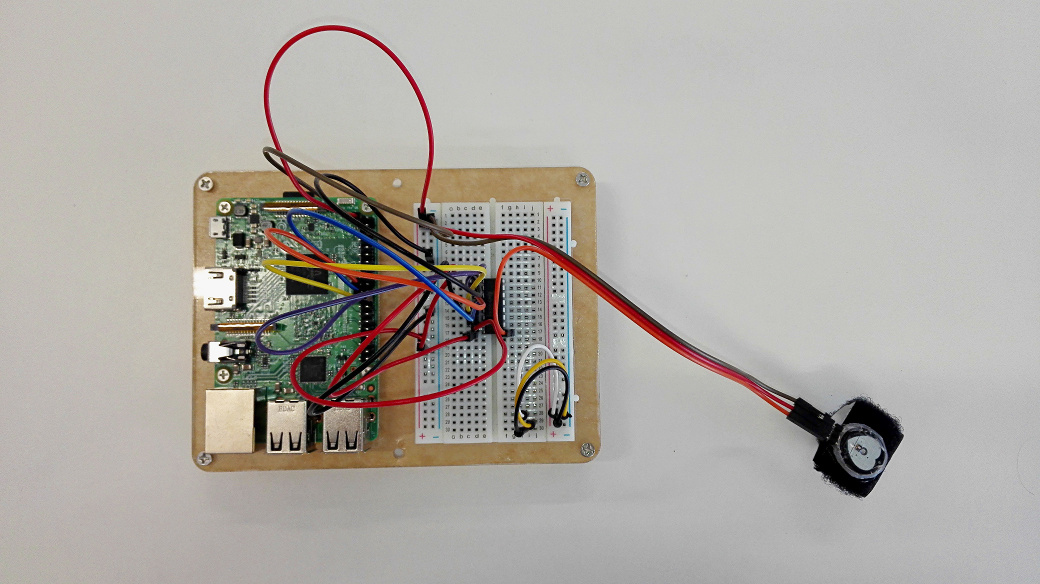
\includegraphics[width=10cm]{img/Chapter4/prototype1_edited.jpg}
% \caption[Prototype setup]{\footnotesize{Prototype setup.}}
% \end{figure}

% \begin{table}[H]
% \centering
% \caption[This is the caption]{ \footnotesize This is the other caption. Since the trial size of the experiments showed is one second, the number of \textit{Target} and \textit{Impostor} data corresponds to number of trials or seconds}
% \label{tab:data_partition}
% \footnotesize{
% \begin{tabular}{@{}llcccc@{}}
% \toprule
% \textbf{Dataset}         & \multicolumn{1}{c}{\textbf{Label}} & \textbf{Train} & \textbf{Validation} & \textbf{Develop} & \textbf{Test} \\ \midrule
% \midrule
% \multirow{3}{*}{First} & Target   & $135$ & $45$  & $30$  & $30$  \\
%                          & Impostor & $5,220$    & $1,740$ & $1,890$   & $2,880$    \\
% \cmidrule(lr){3-5} \cmidrule(l){6-6}
%                          & \#Subjects          & \multicolumn{3}{c}{$31$} & $12$ \\
% \midrule
% \multirow{3}{*}{Second}  & Target   & $144$ & $80$  & $48$  & $48$  \\
%                          & Impostor & $2,014$    & $1,119$    & $1,343$    & $1,545$ \\
% \cmidrule(lr){3-5} \cmidrule(l){6-6}
%                          & \#Subjects   & \multicolumn{3}{c}{$15$} & $5$ \\ 
% \bottomrule
% \end{tabular}
% }
% \end{table}

% \begin{algorithm}
\caption{Temperature-Distributed algorithm}\label{alg:tempdistrib}
\begin{algorithmic}[1]
\Procedure{Temp-Spread}{$GN_i, HN_j, temperatures$}\Comment{Lowest temperature priority}
\State $temperature\_list\gets short(temperatures)$
\State $max_temperature\gets max(temperature_list)$
\State $ThresHold\gets 0.5$
\State $temperature\_impact \gets 0.2$
\For{$GN_i$ in $i=1,8$}\Comment{Iterate every hardware node on the given GN}
\State $it\_temperature \gets temperature\_list(GN_i)$
\State $temp\_weight \gets \frac{max\_temperature-it\_temperature}{max\_temperature}*temperature\_impact$
\State $\omega(Master-GN_i) \gets ThresHold*temp\_weight$
\For{$HN_j$ in $j=1,n$}
\If{$available\_accel_{i,j} > busy\_accel_{i,j}$}
    \State $policy_\omega = \frac{Available HW}{Total HW}*ThresHold$
    \State $\omega(GN_i-HN_{i,j}) \gets ThresHold+policy_\omega$
\Else
    \State $\omega(GN_i - HN_{i,j}) \gets 1$
\EndIf

\EndFor
\EndFor
\State $node \gets find\_djistra\_shortest\_path(Master\_Node, aux\_node)$
\State \textbf{$return node$} $b$\Comment{The gcd is b}
\EndProcedure
\end{algorithmic}
\end{algorithm}

\subsection{Optimization of the code}

The first bottleneck found in the process of computing the histogram was the construction of the matrix $M$ itself. In the first iterations of the code we weren't considering the possibility of parallelizing, or even vectorizing the operations. When speaking of \textit{vectorizing} we refer to the use of numpy arrays and operations, which are optimized for numerical operations.

The initial implementation of the $M$ matrix calculation consisted on computing the matrix elements in a serial way, applying the hankel function to each element of the matrix. The approximate time of computing the whole matrix of dimension $N\times N \approx 700\times 700$ was around 20 seconds. Then, exploiting the fact that the matrix is symmetric, the time was reduced to around 10 seconds.

After this, an arcaic parallelisation scheme was proposed: the matrix was divided in four triangular blocks [make figure], and each block was computed in a different process. This computation was done initializing 4 different jobs with the multiprocessing library, and then joining the results. With this we achieved a time of 2.5 seconds for the whole matrix. Even though, the time was reduced by a factor of 8, it was still the bottleneck of the computation.

Finally, thanks to some training done externally, and by rethinking the way in which the matrix is constructed, the construction stopped being the bottleneck. With the help of the fact that numpy and scipy functions are optimized to work with array-like data, the construction was thought as follows:

\begin{enumerate}
    \item From the list of scatterers (array of dimension $(N,2)$ consisting on 2D vectors representing the coordinates of each scatterer) an upper diagonal matrix (without diagonal) is constructed, consisting on the value of the distance of dispersor $i$ with dispersor $j$. That is:
    \begin{equation}
        \mathcal{D}_{ij}=\begin{cases}
            |r_i-r_j|& i<j\\
            0&else
        \end{cases}
    \end{equation}
    This matrix is computed using numba's njit decorator [ANNEX?]
    \item This matrix is then multiplied by the momentum of the free particle. This basically is an upper triangular matrix that contains the argument of the hankel function.
    \item Then, the hankel function is applied once to the whole matrix, reducing the for loops needed.
    \item The transposed matrix is added to the upper triangular matrix.
    \item Finally, the diagonal is added.
\end{enumerate}


%%% ENVIRONMENT %%%
\clearpage

\section[Environment Impact (Optional)]{{Environment Impact (Optional)}}

{Whether the tasks that have led to the realization of this thesis, as if its results have identifiable environmental
impact, describe it in this section.}

SHOULD I PUT HERE THE STUDY OF EFFICIENCY OF THE SIMULATION?

%%% CONCLUSION AND FUTURE %%%
\clearpage
\section{Conclusions and future development: }

2D SCATTERING IS A WEIRD TOPIC. NEEDS DEVELOPMENT. FEW REFERENCES AND ALL OF THEM DIFFERENT APPROACHES.

%%% BIBLIOGRAPHY %%%
\newpage

\medskip
\bibliographystyle{unsrt}
\bibliography{bibliography.bib}

%%% ANNEX %%%
\clearpage
\newpage

\begin{appendices}

\appendix
\section{Two dimensional scattering: binary collisions}

In the dilute gas, interactions are well described by a binary collision model, where the interaction Hamiltonian is defined as a sum of two-body terms.

\begin{equation}
    \hat{H}_{\text{int}} =\frac{1}{2} \sum_{i \neq j} U({\mathbf{r}}_i - {\mathbf{r}}_j)
\end{equation}

Then it is straightforward that we must begin describing the problem with two bodies interacting via the potential $U(r)$. The study is simplified by the following remarks:

\begin{itemize}
    \item Dominant interactions are spherically symmetric, so that $U(r)$ actually only depends on $r=|\mathbf{r}|$. Angular momenutm is conserved in a collision, allowing the two-body problem to be treated with eigenstates of the operator $\hat{\mathbf{L}}$. This is the principle of development in partial waves, identified by the angular quantum number $l\in\mathbb N$. Note also that for polarized bosons, the symmetrization of the two-body wave function results in only the even values of $l$ being allowed.
    \item Atoms are cold so their thermal wavelength $\lambda_T$ is large compared to the size of the potential, which we call $b$. In other words, the wavevectors $\mathbf{k}$ relevant, which are of the order of $\frac{1}{\lambda_T}$, verifies $kb<<1$. Furthermore, the potential decays rapidly at large distances (short range potential). Those two properties, ensure that the essential properties of the collision are described by the \textit{s-waves}, that is to say the state corresponding to a relative angular momentum $l=0$ between the two collisioned particles.
\end{itemize}

\subsection{Variable separation, diffusion amplitude}

Consider two identical atoms with mass $m$. We can introduce the center of mass variables $\vb{R}$ and $\vb{P}$:

\begin{equation}
    \vb{R} = \frac{1}{2}(\vb{r}_1 + \vb{r}_2) \quad \quad \vb{P} = \vb{p}_1 + \vb{p}_2
\end{equation}

and the relative variables $\vb{r}$ and $\vb{p}$:

\begin{equation}
    \vb{r} = \vb{r}_1 - \vb{r}_2 \quad \quad \vb{p} = \frac{1}{2}(\vb{p}_1 - \vb{p}_2)
\end{equation}

The Hamiltonian of the system can be separated in two terms:

\begin{equation}
    \hat{H} = \hat{H}_{CM}+\hat{H}_{rel}, \quad \quad \hat{H}_{CM} = \frac{\hat{P}^2}{2M}, \quad \quad \hat{H}_{rel} = \frac{\hat{p}^2}{2\mu} + U(\vb{r})
\end{equation}

Where we introduced the total mass $M=2m$ and the reduced mass $\mu = \frac{m}{2}$. The binary collision problem therefore reduces to the problem of a body of reduced mass $\mu$ in the external potential $U(\vb{r})$, described by the Hamiltonian $\hat{H}_{rel}$. This is the problem we will solve in the following.

We will focus on asymptotically free states which describe a diffusion process. the formalism of collision theory tells us that any plane wave $e^{i\vb k\cdot \vb r}$ is an eigenstate of the Hamiltonian

\begin{equation}
    \hat{H}_{rel,0} = \frac{\hat{p}^2}{2\mu}
\end{equation}

With eigenvalue $E_{\vb{k}}=\frac{\hbar^2 k^2}{2\mu}$, then we can associate an eigenstate $\psi_{\vb k}(\vb r)$ of $\hat{H}_{rel}$ with the same energy,

\begin{equation}
    \hat{H}_{rel}\psi_{\vb k}(\vb r) = E_{\vb k}\psi_{\vb k}(\vb r)
\end{equation}

this state is written asymptotically as the sum of the incident plane wave and an outgoing spherical (three-dimensional) or cylindrical (two-dimensional) wave:

\begin{equation}\label{eq:asymptotic_state}
    \begin{cases}
        \text{3D},1\ll kr: & \psi_{\vb k}(\vb r) \sim C_0\biggl \{e^{i\vb k\cdot \vb r} + f(k)\frac{e^{ikr}}{r}\biggr \} \\
        \text{2D},1\ll kr  : & \psi_{\vb k}(\vb r) \sim C_0\biggl \{e^{i\vb k\cdot \vb r} + f(k)\frac{e^{ikr}}{\sqrt{kr}}\biggl [ -\sqrt{\frac{\text{i}}{8\pi}}\biggr ]\biggr \}
    \end{cases}
\end{equation}

Where $C_0$ is a normalization constant. We have taken into account the fact that diffusion takes place essentially in the channel with zero angular momentum (s wave) and therefore we limit ourselves to the case of an isotropic diffused wave. Furthermore, we note that the definition of the diffusion amplitude $f(k)$ is not exactly the same in three and two dimensioins, with the factor $\sqrt{k}$ which apperas explicitly in the two-dimensional case. The definitions adopted here ensures analytical properties that are simple to $f(k)$ [some reference]. Finally, let us point out that the reason for the factor in square brackets in the 2D definition is due to the form found for $f(k)$ in the case of a quasi-2D geometry (more on that later) which will take the form $f(k)\approx \tilde{g}$, where the constant $\tilde{g}$ is the parameter usually used to characterize the strength of interactions in this type of problem. 

The diffusion amplitude $f(k)$ therefore determines the properties of the binary collision. To compute it, we have to take the angular average of the Schrödinger equation, noting that $R_k(r)=\frac{1}{4\pi}\int \psi_{\vb k}(r,\theta,\phi)\sin\theta d\theta d\phi$ in 3D and $R_k=\frac{1}{2\pi}\int \psi_{\vb k}(r,\phi)d\phi$ in 2D. Then, one arrives to the radial Schrödinger equation:

\begin{equation}
    \text{3D:}\qquad \dv[2]{R_k}{r}+\frac{2}{r}\dv{R_k}{r}+\qty[k^2-\frac{2\mu}{\hbar^2}U(r)]R_k = 0
\end{equation}

And 

\begin{equation}
    \text{2D:}\qquad \dv[2]{R_k}{r}+\frac{1}{r}\dv{R_k}{r}+\qty[k^2-\frac{2\mu}{\hbar^2}U(r)]R_k = 0
\end{equation}

Even though the difference between the 3D and the 2D equation appears to be very minor, with only a factor of 2 difference for the first derivative term, we will see that this difference strongly changes the behaviour of the radial function $R_k(r)$ and the diffusion amplitude $f(k)$. Note that the asymtotic behaviour of the radial function $R_k(r)$ is obtained by the angular mean of \cref{eq:asymptotic_state}:

\begin{equation}
    \begin{cases}
        \text{3D},1\ll kr: & R_{k}(r) \sim C_0\biggl \{\frac{\sin(kr)}{kr} + f(k)\frac{e^{ikr}}{r}\biggr \} \\
        \text{2D},1\ll kr  : & R_{k}(r) \sim C_0\biggl \{J_0(kr) + f(k)\frac{e^{ikr}}{\sqrt{kr}}\biggl [ -\sqrt{\frac{\text{i}}{8\pi}}\biggr ]\biggr \}
    \end{cases}
\end{equation}

To simplify our analysis, we will assume that the potential $U(r)$ vanishes beyond the radius $b$. We will focus on the low energy regime $kb\ll 1$, so that there exists an intermediate region of space

\begin{equation}
    b<r\ll k^{-1}
\end{equation}

such that the potential $U(\vb r)$ has no influence and where we can do a developement at small values of $kr$ for diffusion states $\psi_k(r)$. In particular, the incident plane wave $e^{i\vb k\cdot \vb r} \approx 1$ in this intermediate region.

\subsection{The diffusion amplitude in 3D}

In this section, we aim to obtain a solution of the Schrödinger equation with the corresponding asymptotic behaviour. To do this, we will proceed in three steps, which we will then use to compute it in the two-dimensional case:

\begin{enumerate}
    \item \textbf{General solutions in the area $U=0$}. We will place ourselves in the zone $r>b$, where $U$ is negligible. The two functions $\frac{e^{\pm ikr}}{r}$ are exact solutions of the radial equation (as well for $kr\gg 1$ and for $b<r<k^{-1}$), and the general solution is a linear combination of these two functions. In particular, if one looks at the intermediate region $b<r<k^{-1}$, one finds:
    \begin{equation}
        \frac{e^{\pm ikr}}{r}\approx \frac{1\pm ikr}{r}=\frac{1}{r}\pm ik
    \end{equation}

    which, by linear combinations, give a convenient basis of solutions in this region\footnote{That can be infered taking the limit $k\to 0$ $U\to 0$ in the radial function, so that the final equation is $rR''+2R'=0$, which integrates into $R'(r)=\frac{C_2}{r^2}$ where $C_2$ is a constant, and therefore $R(r)=C_1-\frac{C_2}{r}$, where $C_1$ is another constant}:
    \begin{equation}
        R^{(I)}(r)=1\qquad R^{(II)}(r)=\frac{1}{r},
    \end{equation}

    or

    \begin{equation}
        R(r)=C_1-C_2\frac{1}{r},
    \end{equation}

    Where $C_1$ and $C_2$ are constants. The asymptotic shape written in terms of the two functions $\frac{e^{\pm ikr}}{r}$ can be transposed to this intermediate region, since these functions are exact solutions as long as the potential $U$ is negligible and we end up with the form of the radial function:
    \begin{equation}
        R_k(r) = C_1\qty[1+\frac{f(k)}{r}]
    \end{equation}
    \begin{itemize}
        \item A bit more detail in the last calculation:
        
        In this intermediate region, $e^{\pm ikr}\approx 1\pm ikr$. Taking:
        \[R_k(r)\sim C_0\qty[\frac{\sin(kr)}{kr}+f(k)\frac{e^{ikr}}{r}]\] 
        and using $sin(x)=\frac{e^{ix}-e^{-ix}}{2i}$, we get:
        \[R_k(r)\sim C_0\qty[\frac{e^{ikr}-e^{-ikr}}{2ikr}+f(k)\frac{e^{ikr}}{r}]=C_0\qty[\frac{1+ikr-(1-ikr)}{2ikr}+f(k)\frac{1+ikr}{r}]\]
        Then this can be expressed as:
        \[R_k(r)\sim C_0\qty[1+f(k)\qty(\frac{1}{r}\underbrace{+ik}_{??})]\]
        And as we are in this region, $k\to 0$, we can neglect the term $ik$ and we get the expression for $R_{k}(r)$.
    \end{itemize}
    \item \textbf{Zero energy solution}. Let's take $k=0$ in the radial Schrödinger equation and consider the region $r<b$ where $U(r)$ can't be neglected. As it is a second order differential equation, the space solution is of dimension 2. However, we generally find that a single linear combination of solutions is accepatable if we want to respect the regularity of $R_0(r)$ at $r=0$. When we follow this solution to the point $r=b$, where $U$ becomes negligible and then the previous asymptotic form becomes relevant, this linear combination imposes the ratio $\frac{C_2}{C_1}$. Defining the three-dimensional diffusion lenght by this ratio $a=\frac{C_2}{C_1}$, the solution for $E=0$ has the form:
    \begin{equation}
        R_0(r)=C_1\qty[1-\frac{a}{r}]
    \end{equation}
    The diffusioin length is by construction the point in which this asymptotic form vanishes.
    \item \textbf{Connect solutions for low energy} Let's consider now a solution $R_k(r)$ of low energy $kb\ll 1$ and let us place ourselves in the intermediate zone $b<r<k^{-1}$. The comparison of the asymptotic form of $R_k(r)$ with the solution at zero energy, implies a direct link between the diffusion amplitude $f(k)$ and the diffusion length $a$:
    \begin{equation}
        a = -\lim_{k\to 0}f(k)
    \end{equation}

    The total cross section of diffusion by the potential $U(r)$ is the calculated by the balance of probability currents at the input and output and we find $\sigma = 4\pi a^2$. For bosonic particles, the effects of quantum statistics adds a factor of 2 in the result.
\end{enumerate}

\subsection{The diffusion amplitude in 2D}

Proceeding as the 3D case:

\begin{enumerate}
    \item \textbf{General solutions in the area $U=0$}. The 2D case is inherently more complicated than the 3D case, because cylindrical waves $\frac{e^{\pm ikr}}{\sqrt{r}}$ are not exact solutions of the corresponding radial equation for $U=0$. If they were, the lower energy limit would provide the basis of functions $\frac{1}{\sqrt{r}}\pm ik \sqrt{r}$, or the linear combination of $\frac{1}{\sqrt{r}}$ and $\sqrt{r}$. But in the limit $k\to 0$ and $U\to 0$, the radial equation reads $rR''+R'=0$, which integrates into $R'(r)=\frac{C_1}{r}$, where $C_1$ is a constant, and therefore 
    \begin{equation}\label{eq:radial_2D_U0}
    R(r)=C_1\ln r+C_2,
    \end{equation} 
    
    where $C_2$ is another constant. To find this result in a more general framework, we note that the radial equation in 2D for $U=0$ is, in fact, the definition equation for Bessel functions of order 0. Two independent solutions of this equation are the Bessel function of the first kind, $J_0(kr)$, and the Bessel function of the second kind, $Y_0(kr)$. The behavior of the functions $J_0(kr)$ and $Y_0(kr)$ are known for big and small values of $kr$:

    \begin{align*}
        kr\gg 1: & \quad J_0(kr)\sim \sqrt{\frac{2}{\pi kr}}\cos(kr-\frac{\pi}{4}) \\
        & \quad Y_0(kr)\sim \sqrt{\frac{2}{\pi kr}}\sin(kr-\frac{\pi}{4})
    \end{align*}

    and

    \begin{align*}
        kr\ll 1: & \quad J_0(kr)\sim 1 \\
        & \quad Y_0(kr)\sim \frac{2}{\pi} \ln(\eta kr)
    \end{align*}

    Where $\eta\equiv \frac{e^\gamma}{2}$, with $\gamma$ the Euler-Mascheroni constant. In particular, every linear combination of $J_0(kr)$ and $Y_0(kr)$ at $kr\ll 1$ is a solution of the described form.

    \item \textbf{Zero energy solution}. For $k=0$, and with the presence of a potential $U(r)$, the space of general solutions $R_0(r)$ is of dimension 2. However, the regularity of $R_0(r)$ at $r=0$ imposes a restriction on the linear combination of solutions. When we extend it beyond the radius $r=b$ this linear combination is connected to a particular linear combination of the type shown in \cref{eq:radial_2D_U0}, which can be written as:
    \begin{equation}
        r>b:\quad R_0(r)=C_1\ln(\frac{r}{a_2})
    \end{equation}

    Where $a_2\equiv e^{-\frac{C_2}{C_1}}$ \color{red}Isn't it our definition $a_{eff}=a_2\eta$? \color{black} is the diffusion length in two dimensions.
    \item \textbf{Connect solutions for low energy}. Moving to the case in which $k$ is not zero but remains very small in front of $b^{-1}$. To form an outgoing cylindrical wave, we see from the behaviours of $J_0(kr)$ and $Y_0(kr)$ that we must take a function proportional to the linear combination $J_0(kr)+\text{i}Y_0(kr)\equiv H_0^{(1)}(kr)$. More precisely, we will choose:
    
    \begin{equation}
        \text{2D, } 1\ll kr: \quad \frac{1}{4\text{i}}\qty[J_0(kr)+\text{i}Y_0(kr)]\sim \frac{e^{ikr}}{\sqrt{kr}}\qty[-\sqrt{\frac{\text{i}}{8\pi}}]
    \end{equation}

    \begin{itemize}
        \item A bit more detail in the last calculation:
        Using the expressions for $J_0(kr)$ and $Y_0(kr)$, in the limit $kr\gg 1$ we have:
        \begin{align*}
            \frac{1}{4\text{i}}\qty[J_0(kr)+\text{i}Y_0(kr)]&= \frac{1}{4\text{i}}\qty[\sqrt{\frac{2}{\pi kr}}\cos(kr-\frac{\pi}{4})+\text{i}\sqrt{\frac{2}{\pi kr}}\sin(kr-\frac{\pi}{4})] \\
            & = \frac{1}{4\text{i}}\sqrt{\frac{2}{\pi kr}}\qty[\cos(kr-\frac{\pi}{4})+\text{i}\sin(kr-\frac{\pi}{4})] \\
            & = \frac{1}{4\text{i}}\sqrt{\frac{2}{\pi kr}}e^{i(kr-\frac{\pi}{4})} 
             = \sqrt{\frac{2}{16\pi \text{i}}}\frac{e^{ikr}}{\sqrt{kr}}\underbrace{e^{-i\frac{\pi}{4}}}_{??}\\
            & = -\sqrt{\frac{\text{i}}{8\pi}}\frac{e^{ikr}}{\sqrt{kr}}e^{-i\frac{\pi}{4}}
        \end{align*}
    \end{itemize}
    Where we can recognize the factor we introduced with the diffusion amplitude. For $r>b$, the desired radial function is therefore of the type
    \begin{equation}
        R_k(r)=C_0\qty[J_0(kr)+\frac{f(k)}{4\text{i}}H_0^{(1)}(kr)]
    \end{equation}

    In the intermediate region $b<r<k^{-1}$, this linear combination becomes:

    \begin{equation}
        R_k(r)=C_0\qty[+\frac{f(k)}{4\text{i}}\qty(1+\text{i}\frac{2}{\pi}\ln(\eta kr))]
    \end{equation}

    Which, in the limit of $k\to 0$, the diffusion amplitude is given by:

    \begin{equation}
        f(k)=-4\text{i}\frac{1}{1+\text{i}\frac{2}{\pi}\ln(\eta k a_2)}=\frac{1}{-\frac{1}{2\pi}\ln(\eta k a_2)+\frac{\text{i}}{4}}
    \end{equation}

    So that we recover the form found earlier $C_1\ln(\frac{r}{a_2})$ with, in particular, $R_k(r)=0$ at $r=a_2$.

    Note that the diffusion amplitude $f(k)$ tends towards 0 at small $k$, unlike the 3D case where it tended towards a finite limit equal to $-a$. Furthermore, the total cross section of diffusion by the potential $U(r)$ is also calculated here by a balance of the probability currents at the input and output. We find $\sigma(k)=\frac{|f(k)|^2}{4k}$, which has the dimension of length and diverges gradually with the decrease of $k$.
\end{enumerate}



\appendix
\section{Quantum mechanics formalism}

Quantum mechanics is a fundamental theory in physics that describes the behavior of particles at the atomic and subatomic scales. The theory is based on the postulates of quantum mechanics. TODO(?)

\subsection{Green's function in the mathematical context}

This work has been developed using the \textit{Green's function method} for solving non-homogeneous differential equations. 

Given a differential equation of the form $\mathcal L u(x) = f(x)$, where $\mathcal L$ is a \textit{linear differential operator} acting on distributions over a subset $\Omega$ of the euclidean space $\mathbb R^n$, the Green's function at point $s\in \Omega$ is defined as:

\begin{equation}
    \mathcal L G(x,s)=\delta(x-s)
\end{equation}

These functions are a useful tool in wave mechanics, as they can be used to solve differential equations of the form:

\begin{equation}\label{eq:diffeqprob}
    \mathcal L u(x)=f(x)
\end{equation}

\begin{theorem}
    Given a Green's function $G(x,s)$ that corresponds to the linear differential operator $\mathcal{L}(x)$, the solution of the problem \ref{eq:diffeqprob} is given by:
    \begin{equation}
        u(x)=\int_\Omega G(x,s) f(s) ds
    \end{equation}
\end{theorem}

\begin{proof}
    Starting from the definition of the Green's function, we can integrate by $\int_\Omega f(s)ds$:
    \begin{equation}
        \int_\Omega \mathcal L (x) G(x,s)f(s)ds=\int_\Omega\delta (x-s)f(s)ds
    \end{equation}

    Given that $\mathcal{L}$ is linear in $x$, and using the properties of the $\delta$ distribution, we have:
    \begin{equation}
        \mathcal{L}\int_\Omega G(x,s)f(s)ds=f(x)
    \end{equation}

    And one can identify that:
    \begin{equation}
        u(x)=\int_\Omega G(x,s)f(s)ds
    \end{equation}
    
    Where the Green's function $G(x,s)$ satisfies the same boundary conditions as $u(x)$.
\end{proof}

An important fact to notice is that if the differential operator's coefficients are constant with respect of the independent variable $x$, the system is transnational invariant and the Green's function is just a function of a single variable:

\begin{equation}
    G(x,s)=G(x-s)
\end{equation}

\subsection{Green's function in quantum mechanics: The single particle propagator}

Knowing the Green's function method, we can apply it to the well known time-independent Schrödinger equation in the position representation. Given a Hamiltonian $H_0(\vb r)$, the eigenstates of which are known, we can write the Schrödinger equation as:

\begin{equation}
    \qty(H_0(\vb r)+V(\vb r)){\Psi_E(\vb r)}=E{\Psi_E(\vb r)}
\end{equation}

This is a useful representation of the scattering problems, where $H_0(\vb r)$ is the initial Hamiltonian and $V(\vb r)$ would be the potential that scatters the particles. We can rewrite the equation as:

\begin{equation}
    \qty(E-H_0(\vb r)){\Psi_E(\vb r)}=V(\vb r){\Psi_E(\vb r)}
\end{equation}

Which is a non-homogeneous differential equation of the form of \cref{eq:diffeqprob}, where the source term is $V(x){\Psi_E(\vb r)}$. The Green's function for the time independent Schrödinger equation is defined as:

\begin{equation}
    \qty(E-H_0(\vb r))G_0(\vb r,\vb s;E)=\delta(\vb r-\vb s)
\end{equation}

Where it is natural to define the inverse of $G_0(\vb r,\vb s)$ as the operator $E-H_0(\vb r)$. To be rigurous, the inverse of the Green's function is defined as:

\begin{equation}
    G_0^{-1}(\vb r,\vb s;E)=\qty(E-H_0(\vb r))\delta(\vb r-\vb s)\equiv G_0^{-1}(\vb r)
\end{equation}

This representation is just a way of saying that the inverse of the Green's function is diagonal in the position representation. With this definition, we can see that it is in fact the inverse of the Green's function:

\begin{equation}
    \int_\Omega G_0^{-1}(\vb r,\vb s;E)G_0(\vb s,\vb y;E)ds=\int_\Omega \qty(E-H_0(\vb r))\delta(\vb r-\vb s)G_0(\vb s,\vb y;E)ds=\qty(E-H_0(\vb r))G_0(\vb r,\vb y;E)=\delta(\vb r-\vb y)
\end{equation}

Then, the Schrödinger equation can be rewritten as:

\begin{equation}\label{eq:schrod_eq_green}
    \qty(G_0^{-1}(\vb r;E)-V(\vb r)){\Psi_E(\vb r)}=0
\end{equation}

With:

\begin{equation}\label{eq:inverse_green}
    G_0^{-1}(\vb r;E)G_0(\vb r,\vb y;E)=\delta(\vb r-\vb y)
\end{equation}

\begin{proposition}
    The solution of the Schrödinger equation is given by:
    \begin{equation}\label{eq:schrod_eq_sol}
        \Psi_E(\vb r)=\Psi_E^0(\vb r)+\int_\Omega G_0(\vb r,\vb s;E)V(\vb s){\Psi_E(\vb s)}d\vb s
    \end{equation}

    Where $\Psi_E^0(\vb r)$ is the solution of the homogeneous equation.
\end{proposition}

\begin{proof}
    We can substitute the proposed solution (\cref{eq:schrod_eq_sol}) into the Schrödinger equation \cref{eq:schrod_eq_green}:
    \begin{equation}
        \qty(G_0^{-1}(\vb r;E)-V(\vb r))\qty(\Psi_E^0(\vb r)+\int_\Omega G_0(\vb r,\vb s;E)V(\vb s){\Psi_E(\vb s)}d\vb s)=0
    \end{equation}

    Using the definition of $\Psi_E^0(\vb r)$, we can see that:
    \[G_0^{-1}(\vb r;E)\Psi_E^0(\vb r)=0\]
    As this is just the homogeneous Schrödinger equation. Then, the expression simplifies to:
    \begin{equation}
        \qty(G_0^{-1}(\vb r;E)-V(\vb r))\int_\Omega G_0(\vb r,\vb s;E)V(\vb s){\Psi_E(\vb s)}d\vb s=V(\vb r)\Psi_E^0(\vb r)
    \end{equation}

    Grouping all terms with the potential $V(\vb r)$, we have:

    \begin{equation}
        G_0^{-1}(\vb r;E)\qty(\int_\Omega G_0(\vb r,\vb s; E)V(\vb s)\Psi_E(\vb s)d\vb s)=V(\vb r)\underbrace{\qty(\Psi_E^0(\vb r)+\int_\Omega G_0(\vb r,\vb s; E)V(\vb s)\Psi_E(\vb s)d\vb s)}_{\Psi_E(\vb r)}
    \end{equation}

    And, using \cref{eq:inverse_green}, we have:
    \begin{equation}
        \int_\Omega \underbrace{G_0^{-1}(\vb r; E)G_0(\vb r,\vb s; E)}_{\delta(\vb r-\vb s)}V(\vb s)\Psi_E(\vb s)d\vb s=V(\vb r)\Psi_E(\vb r)\qedhere
    \end{equation}
\end{proof}

For the time-dependent Schrödinger equation, problem is formulated as:

\begin{equation}\label{eq:td_schrod_eq}
    \qty(i\partial_t-H_0(\vb r)-V(\vb r)){\Psi(\vb r,t)}=0
\end{equation}

Now we can define two operators as follows:

\begin{subequations}
    \begin{align}
        \qty(i\partial_t-H_0(\vb r))G_0(\vb r,\vb s;t-t')&=\delta(\vb r-\vb s)\delta(t-t')
        \\
        \qty(i\partial_t-H_0(\vb r)-V(\vb r))G(\vb r,\vb s;t-t')&=\delta(\vb r-\vb s)\delta(t-t')
    \end{align}
\end{subequations}

And, following the diagonal notation, we can identify the inverse operators as:

\begin{align}
    G_0^{-1}(\vb r,;t)&=i\partial_t-H_0(\vb r)
    \\
    G^{-1}(\vb r;t)&=i\partial_t-H_0(\vb r)-V(\vb r)
\end{align}

Then, we can express the self-consistent equation as:

\begin{align}
    \Psi(\vb r,t)=\Psi^0(\vb r,t)+\int d\vb r' \int dt' G_0(\vb r,\vb r';t-t')V(\vb r')\Psi(\vb r',t')\label{eq:free_prop_td}\\
    \Psi(\vb r,t)=\Psi^0(\vb r,t)+\int d\vb r' \int dt' G(\vb r,\vb r';t-t')V(\vb r')\Psi^0(\vb r',t')\label{eq:full_prop_td}
\end{align}

With these two equations, one can derive the Dyson equation for the Green's function, which is a fundamental equation in quantum mechanics. Dropping the integrals from \cref{eq:free_prop_td}, we have:

\begin{align}
    \nonumber \Psi &= \Psi^0 + G_0V\Psi^0+ G_0VG_0V\Psi^0+G_0VG_0VG_0V\Psi^0+\ldots\\
    &= \Psi^0 + (G_0+G_0VG_0+G_0VG_0VG_0+\ldots)V\Psi^0
\end{align}

And comparing it with \cref{eq:full_prop_td}, we can express the operator $G$ as:

\begin{align}
    G &= G_0 + G_0VG_0 + G_0VG_0VG_0 + \ldots\\
    &=G_0 + G_0V (G_0+G_0VG_0+\ldots)
\end{align}

Wich is just the Dyson equation:

\begin{equation}
    G = G_0 + G_0VG
\end{equation}

This new operator $G$ is often called the \textbf{propagator} of the system. This can be seen starting from the time-dependent Schrödinger equation. For this derivation we will use Dirac notation, where the state of the system is represented by a ket $\ket{\alpha,t_0;t}$, where $\alpha$ is the state of the system and $t_0$ is the initial time. The time-dependent Schrödinger equation can be written as:

\begin{equation}
    i\hbar\partial_t\ket{\alpha,t_0;t}=\hat H\ket{\alpha,t_0;t}
\end{equation}

Where $\hat H=H_0+V$ is the Hamiltonian operator of the system. The solution of this equation is given by the operator $\hat U(t,t_0) = e^{-\frac{i}{\hbar}\hat H(t-t_0)}$. Following Dirac notation, the wave function can be written as:

\begin{equation}
    \Psi(\vb r,t)=\bra{\vb r}\hat U(t,t_0)\ket{\Psi(t_0)}
\end{equation}

SEE THIS KERNEL AS THE PROPAGATOR (MANY BODY QUANTUM THEORY EXPOSED!)





\end{appendices}

\end{document}
